\textbf{(a) Use Monte Carlo simulation to estimate the probability that, if the dice are rolled, the sum of the two up-faces will be 7.\\\\}
\begin{lstlisting}[style=CStyle]
/**
 * Homework 2.3
 * EECE 5643 - Simulation and Performance Evaluation
 * Author: Harrison Sun
 * Email: sun.har@northeastern.edu
 */

#define ONEFACEWEIGHT	1
#define OTHERWEIGHT		2
#define SIXFACEWEIGHT	4
#define DEFAULTSEED		0L
#define NUMRUNS			1000000L

#include <exception>
#include <iostream>
#include <stdlib.h>
#include "c_lib/rng.h"

/* Dice Weights */																																					
double oneFaceWeight{ ONEFACEWEIGHT };																																
double otherFaceWeight{ OTHERWEIGHT };																																
double sixFaceWeight{ SIXFACEWEIGHT };																														
/* TOTAL WEIGHT */																																					
double totalWeight{ oneFaceWeight + sixFaceWeight + 4 * otherFaceWeight };																							

/* Dice Probabilities */																																			
double p1 = oneFaceWeight / totalWeight;																															
double pOther = otherFaceWeight / totalWeight;																														
double p6 = sixFaceWeight / totalWeight;																																	
/* Define the thresholds */																																			
double threshold1 = p1;																																				
double threshold2 = threshold1 + pOther;																															
double threshold3 = threshold2 + pOther;																															
double threshold4 = threshold3 + pOther;																															
double threshold5 = threshold4 + pOther;																													
double threshold6 = threshold5 + p6;		/* threshold6 should be equal to 1 */	


/**
 * int Throw_Die(void)
 * 
 * @param void
 * 
 * @return int - the number of the face of the die
 * 
 * This function simulates the throwing of a die. It returns the number of the face of the die.
 */

int Throw_Die(void)
{
	/* Roll the die */
	double r = Random();
	int die{};
	if (r < threshold1)
	{
		die = 1;
	}
	else if (r < threshold2)
	{
		die = 2;
	}
	else if (r < threshold3)
	{
		die = 3;
	}
	else if (r < threshold4)
	{
		die = 4;
	}
	else if (r < threshold5)
	{
		die = 5;
	}
	else if (r < threshold6)
	{
		die = 6;
	}
	else
	{
		std::cerr << "Error: Random number is greater than 1." << std::endl;
		throw std::logic_error("My code is broken. This really shouldn't happen.");
	}
	return die;
}

/**
 * int main()
 * 
 ************* Terminal Arguments *************
 * @param int argc - number of arguments      *
 * @param char* argv[] - array of arguments   *
 **********************************************
 * 
 * @return int - 0 if successful
 * 
 * This is the main function. It uses a Monte Carlo Simulation to estimate the probability that, if weighted dice are rolled, the sum of the two up-faces will be 7.
 */

int main(int argc, char* argv[])
{
	/* Seed definition */
	long seed = (argc > 1) ? atol(argv[1]) : DEFAULTSEED;

	/* Number of runs */
	long num_runs = (argc > 2) ? atol(argv[2]) : NUMRUNS;
	
	/* Random Number Generator */
	PutSeed(seed);
	
	/* Number of times the sum of the two up-faces is 7 */
	long num_7{ 0 };

	/* Roll the dice twice and add the faces together */
	for (int i = 0; i < num_runs; ++i)
	{
		/* Try-Catch Block to catch exceptions (Sum(Pr) != 1) */
		try 
		{
			num_7 = (Throw_Die() + Throw_Die() == 7) ? ++num_7 : num_7;
		}
		catch (const std::logic_error& error)
		{
			std::cerr << error.what() << std::endl;
			return -1;
		}
	}

	/* Print the results */
	std::cout << "The probability that the sum of the two up-faces is 7 is " << (double)num_7 / num_runs << std::endl;

	return 0;
}
\end{lstlisting}
\vspace{50pt}
Terminal Outputs:\\\\
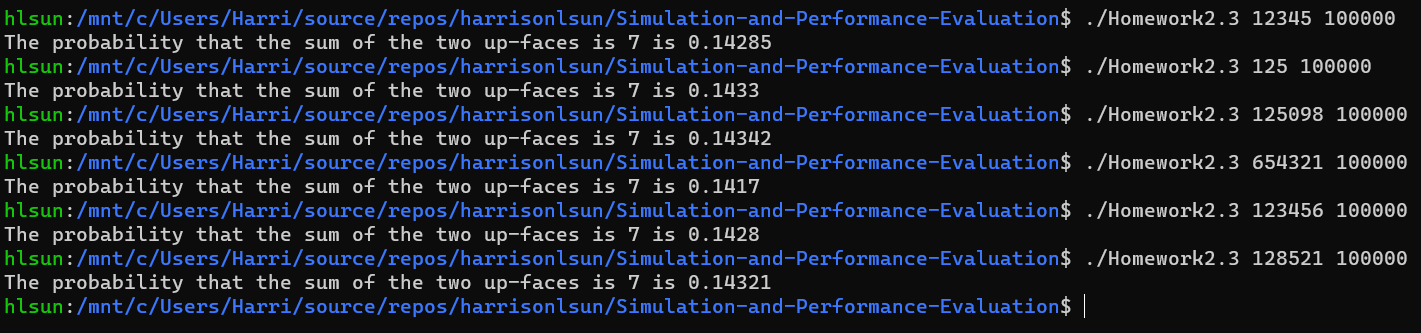
\includegraphics[scale=0.55]{Sections/H2_3.png}\\\\